\section{Theorie}
\label{sec:Theorie}
\subsection{Die Austrittsarbeit der Leitungselektronen}
Metalle sind charakterisiert durch eine sehr gute elektrische Leitfähigkeit. Diese ist
durch die zu einem Gitter angeordneten ionisierten Atome im Metall zu erklären. Die
im Kraftfeld der Ionen befindlichen Elektronen sind als Leitungselektronen nicht mehr
einem Atom zuzuordnen. Die Leitungselektronen sind freibeweglich im Potential $\xi$ des
elektrischen Felds, welches näherungsweise als konstant angenommen werden kann. Ein
Modell, das diesen Zustand darstellt ist der Potentialtopf.
\begin{figure}[H]
    \begin{center}
    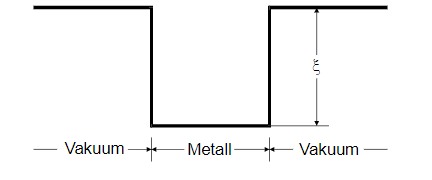
\includegraphics[width = 8cm, height= 3.5cm]{Potentialtopf.png}
    \caption{Potentialtopfmodell.\protect\cite{AL}}
    \end{center}
    \label{fig:Potentialtopf}
    \end{figure}
    \noindent
Damit ein Elektron dieses Potential und damit das Metall verlassen kann, muss es
die sogenannte Austrittsarbeit $e_0 \xi$ leisten. Erklärungen dafür liefert die Quantentheorie.
Elektronen können nur diskrete Energiewerte annehmen. Ein Energiezustand kann laut
dem Pauli-Prinzip nur von einem Elektron besetzt werden, da sie zu den Spin-1/2-Teilchen
gehören. Die Aufenthaltswahrscheinlichkeit ein Elektron in einem Zustand zu finden, ist
durch die Fermi-Dirac-Verteilung gegeben
\begin{equation}
   f(E)=\frac{1}{\text{exp}\Bigl(\frac{E-\zeta}{k_B T}\Bigr)+1}\\
   \end{equation}
\noindent mit $\zeta$ der Fermischen Grenzenergie. Für Zimmertemperatur gilt $\zeta \gg k_b T$ für alle Metalle.
Um ein Metall zu verlassen benötigt ein Elektron also eine Energie von mindestens $\zeta +e_0 \xi$.
Auch für hohe Temperaturen liegt dieser Energiewert weit über $k_bT$, weshalb folgende
Näherung angenommen wird.
\begin{equation}
    f(E)=\text{exp}\Bigl(\frac{\zeta - E}{k_B T}\Bigr)\\
    \end{equation}
\subsection{Die Sättigungsstromdichte der thermischen Elektronenemission}
Die Sättigungsstromdichte $j_s$ beschreibt die Zahl der Elektronen, die pro Zeit- und
Flächeneinheit aus einer Metalloberfläche austreten in Abhängikeit von der Temperatur.
Sie wird mit der Richardson-Gleichung berechnet
\begin{equation}
    j_S(T)=4\pi \frac{e_0m_0k^2_B}{h^3}T^2 \text{exp}\Bigl(-\frac{e_0\xi}{k_BT}\Bigr)\\
    \end{equation}
\subsection{Die Hochvakuum-Diode}
Da die aus einer Metalloberfläche austretenden Elektronen mit Gasmolekülen wechselwirken, kann die Sättigungsstromdichte nur in einem Hochvakuum gemessen werden.
Experimentell lässt sich dies mit einer Hochvakuumdiode realisieren. Sie besteht aus
einem Glaskörper, in dem sich eine Glühkathode(Wolfram) und gegenüberliegend einer
Anode befinden. Durch eine angelegte Heizspannung kann der Draht der Glühkathode
auf Temperaturen von 1000 K bis 3000 K erhitzt werden. Die austretenden Elektronen
werden dann über eine Saugspannung zur Anode beschleunigt.
\begin{figure}[H]
    \begin{center}
    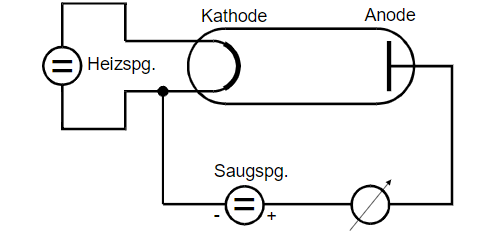
\includegraphics[width = 9cm, height= 5cm]{Hochvakuumdiode.png}
    \caption{Aufbau einer Hochvakuumdiode.\protect\cite{AL}}
    \end{center}
    \label{fig:Hochvakuumdiode}
    \end{figure}
    \noindent
Die Kennlinie einer Hochvakuumdiode lässt sich in drei Bereiche einteilen. Das erste
Gebiet ist das Anlaufstromgebiet(exponentieller Zusammenhang zwischen Strom und
Potential), das zweite wird Raumladungsgebiet ($j \propto V^{3/2}$) genannt und das dritte wird
als Sättigungsstromgebiet(Strom ist nur von der Temperatur abhängig) bezeichnet.
\begin{figure}[H]
    \begin{center}
    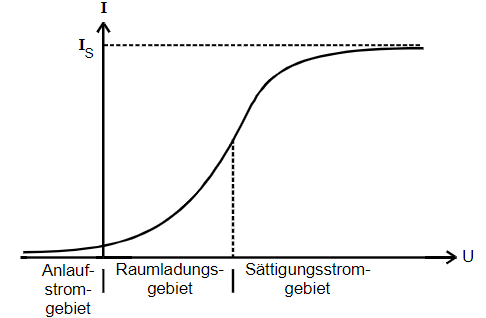
\includegraphics[width = 10cm, height= 6.5cm]{KennlinienHochvakuum.png}
    \caption{Kennlinie einer Hochvakuumdiode.\protect\cite{AL}}
    \end{center}
    \label{fig:KennlinienHochvakuum}
    \end{figure}
    \noindent
\subsection{ Raumladung und das Langmuir-Schottkysche Raumladungsgesetz}
Es fällt auf, dass der gemessene Diodenstrom kleiner ist als der zu erwartende Sättigungsstrom. Erklärt wird dies durch die Elektronen, die bereits aus der Kathode ausgetreten
sind. Jene erzeugen eine ortsabhängig Raumladungsdichte $\rho$, die das elektrische Feld
abschirmt. Nicht alle ausgetretenen Elektronen erreichen die Anode, das Ohmsche Gesetz
verliert in diesem Bereich seine Gültigkeit. Aus dem Zusammenhang zwischen Anodenspannung und -strom im Ladungsbereich, der Poisson-Gleichung
\begin{equation}
\Delta V = - \frac{1}{\epsilon _0} \rho\\
\end{equation}
\noindent
folgt das Langmuir-Schottkysche Raumladungsgesetz
\begin{equation}
j= \frac{4}{9} \epsilon_0 \sqrt{2e_0/m_0} \frac{V^{3/2}}{a}\\
\end{equation}
\noindent $V$ beschreibt die Anodenspannung, $a$ die Entfernung zur Kathode und $m_0$ die Ruhemasse
des Elektrons.
\subsection{Anlaufstromgebiet}
Liegt zwischen Anode und Kathode keine Spannung an, so kann trotzdem ein geringer
Strom gemessen werden, der sogenannte Anlaufstrom. Dieser resultiert aus der kinetischen
Restenergie, die einige Elektronen nach dem Austritt noch besitzen. Um die Anode
zu erreichen, benötigen sie eine Energie, die größer ist als $e_0\Phi_A+e_0V$ mit $\Phi_A$, der
Austrittsarbeit. Für die Stromdichte im Anlaufgebiet gilt dann
\begin{equation}
    j(V)= j_0 \text{exp}\Bigl( - \frac{e_0\Phi_A+e_0V}{k_BT}\Bigr)= \text{const} \cdot \text{exp}\Bigl(-\frac{e_0V}{k_BT}\Bigr) \\
\end{equation}
\begin{figure}[H]
    \begin{center}
    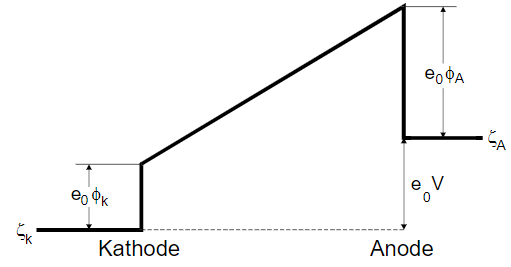
\includegraphics[width = 10.5cm, height= 5.5cm]{Anlaufstromgebiet.png}
    \caption{Potentialverhältnisse in einer Hochvakuumdiode im Bereich ihres Anlaufstromgebietes.\protect\cite{AL}}
    \end{center}
    \label{fig:Anlaufgebiet}
    \end{figure}
    \noindent
